% Options for packages loaded elsewhere
\PassOptionsToPackage{unicode}{hyperref}
\PassOptionsToPackage{hyphens}{url}
\PassOptionsToPackage{dvipsnames,svgnames,x11names}{xcolor}
%
\documentclass[
  letterpaper,
  DIV=11,
  numbers=noendperiod]{scrartcl}

\usepackage{amsmath,amssymb}
\usepackage{iftex}
\ifPDFTeX
  \usepackage[T1]{fontenc}
  \usepackage[utf8]{inputenc}
  \usepackage{textcomp} % provide euro and other symbols
\else % if luatex or xetex
  \usepackage{unicode-math}
  \defaultfontfeatures{Scale=MatchLowercase}
  \defaultfontfeatures[\rmfamily]{Ligatures=TeX,Scale=1}
\fi
\usepackage{lmodern}
\ifPDFTeX\else  
    % xetex/luatex font selection
\fi
% Use upquote if available, for straight quotes in verbatim environments
\IfFileExists{upquote.sty}{\usepackage{upquote}}{}
\IfFileExists{microtype.sty}{% use microtype if available
  \usepackage[]{microtype}
  \UseMicrotypeSet[protrusion]{basicmath} % disable protrusion for tt fonts
}{}
\makeatletter
\@ifundefined{KOMAClassName}{% if non-KOMA class
  \IfFileExists{parskip.sty}{%
    \usepackage{parskip}
  }{% else
    \setlength{\parindent}{0pt}
    \setlength{\parskip}{6pt plus 2pt minus 1pt}}
}{% if KOMA class
  \KOMAoptions{parskip=half}}
\makeatother
\usepackage{xcolor}
\setlength{\emergencystretch}{3em} % prevent overfull lines
\setcounter{secnumdepth}{-\maxdimen} % remove section numbering
% Make \paragraph and \subparagraph free-standing
\makeatletter
\ifx\paragraph\undefined\else
  \let\oldparagraph\paragraph
  \renewcommand{\paragraph}{
    \@ifstar
      \xxxParagraphStar
      \xxxParagraphNoStar
  }
  \newcommand{\xxxParagraphStar}[1]{\oldparagraph*{#1}\mbox{}}
  \newcommand{\xxxParagraphNoStar}[1]{\oldparagraph{#1}\mbox{}}
\fi
\ifx\subparagraph\undefined\else
  \let\oldsubparagraph\subparagraph
  \renewcommand{\subparagraph}{
    \@ifstar
      \xxxSubParagraphStar
      \xxxSubParagraphNoStar
  }
  \newcommand{\xxxSubParagraphStar}[1]{\oldsubparagraph*{#1}\mbox{}}
  \newcommand{\xxxSubParagraphNoStar}[1]{\oldsubparagraph{#1}\mbox{}}
\fi
\makeatother

\usepackage{color}
\usepackage{fancyvrb}
\newcommand{\VerbBar}{|}
\newcommand{\VERB}{\Verb[commandchars=\\\{\}]}
\DefineVerbatimEnvironment{Highlighting}{Verbatim}{commandchars=\\\{\}}
% Add ',fontsize=\small' for more characters per line
\usepackage{framed}
\definecolor{shadecolor}{RGB}{241,243,245}
\newenvironment{Shaded}{\begin{snugshade}}{\end{snugshade}}
\newcommand{\AlertTok}[1]{\textcolor[rgb]{0.68,0.00,0.00}{#1}}
\newcommand{\AnnotationTok}[1]{\textcolor[rgb]{0.37,0.37,0.37}{#1}}
\newcommand{\AttributeTok}[1]{\textcolor[rgb]{0.40,0.45,0.13}{#1}}
\newcommand{\BaseNTok}[1]{\textcolor[rgb]{0.68,0.00,0.00}{#1}}
\newcommand{\BuiltInTok}[1]{\textcolor[rgb]{0.00,0.23,0.31}{#1}}
\newcommand{\CharTok}[1]{\textcolor[rgb]{0.13,0.47,0.30}{#1}}
\newcommand{\CommentTok}[1]{\textcolor[rgb]{0.37,0.37,0.37}{#1}}
\newcommand{\CommentVarTok}[1]{\textcolor[rgb]{0.37,0.37,0.37}{\textit{#1}}}
\newcommand{\ConstantTok}[1]{\textcolor[rgb]{0.56,0.35,0.01}{#1}}
\newcommand{\ControlFlowTok}[1]{\textcolor[rgb]{0.00,0.23,0.31}{\textbf{#1}}}
\newcommand{\DataTypeTok}[1]{\textcolor[rgb]{0.68,0.00,0.00}{#1}}
\newcommand{\DecValTok}[1]{\textcolor[rgb]{0.68,0.00,0.00}{#1}}
\newcommand{\DocumentationTok}[1]{\textcolor[rgb]{0.37,0.37,0.37}{\textit{#1}}}
\newcommand{\ErrorTok}[1]{\textcolor[rgb]{0.68,0.00,0.00}{#1}}
\newcommand{\ExtensionTok}[1]{\textcolor[rgb]{0.00,0.23,0.31}{#1}}
\newcommand{\FloatTok}[1]{\textcolor[rgb]{0.68,0.00,0.00}{#1}}
\newcommand{\FunctionTok}[1]{\textcolor[rgb]{0.28,0.35,0.67}{#1}}
\newcommand{\ImportTok}[1]{\textcolor[rgb]{0.00,0.46,0.62}{#1}}
\newcommand{\InformationTok}[1]{\textcolor[rgb]{0.37,0.37,0.37}{#1}}
\newcommand{\KeywordTok}[1]{\textcolor[rgb]{0.00,0.23,0.31}{\textbf{#1}}}
\newcommand{\NormalTok}[1]{\textcolor[rgb]{0.00,0.23,0.31}{#1}}
\newcommand{\OperatorTok}[1]{\textcolor[rgb]{0.37,0.37,0.37}{#1}}
\newcommand{\OtherTok}[1]{\textcolor[rgb]{0.00,0.23,0.31}{#1}}
\newcommand{\PreprocessorTok}[1]{\textcolor[rgb]{0.68,0.00,0.00}{#1}}
\newcommand{\RegionMarkerTok}[1]{\textcolor[rgb]{0.00,0.23,0.31}{#1}}
\newcommand{\SpecialCharTok}[1]{\textcolor[rgb]{0.37,0.37,0.37}{#1}}
\newcommand{\SpecialStringTok}[1]{\textcolor[rgb]{0.13,0.47,0.30}{#1}}
\newcommand{\StringTok}[1]{\textcolor[rgb]{0.13,0.47,0.30}{#1}}
\newcommand{\VariableTok}[1]{\textcolor[rgb]{0.07,0.07,0.07}{#1}}
\newcommand{\VerbatimStringTok}[1]{\textcolor[rgb]{0.13,0.47,0.30}{#1}}
\newcommand{\WarningTok}[1]{\textcolor[rgb]{0.37,0.37,0.37}{\textit{#1}}}

\providecommand{\tightlist}{%
  \setlength{\itemsep}{0pt}\setlength{\parskip}{0pt}}\usepackage{longtable,booktabs,array}
\usepackage{calc} % for calculating minipage widths
% Correct order of tables after \paragraph or \subparagraph
\usepackage{etoolbox}
\makeatletter
\patchcmd\longtable{\par}{\if@noskipsec\mbox{}\fi\par}{}{}
\makeatother
% Allow footnotes in longtable head/foot
\IfFileExists{footnotehyper.sty}{\usepackage{footnotehyper}}{\usepackage{footnote}}
\makesavenoteenv{longtable}
\usepackage{graphicx}
\makeatletter
\def\maxwidth{\ifdim\Gin@nat@width>\linewidth\linewidth\else\Gin@nat@width\fi}
\def\maxheight{\ifdim\Gin@nat@height>\textheight\textheight\else\Gin@nat@height\fi}
\makeatother
% Scale images if necessary, so that they will not overflow the page
% margins by default, and it is still possible to overwrite the defaults
% using explicit options in \includegraphics[width, height, ...]{}
\setkeys{Gin}{width=\maxwidth,height=\maxheight,keepaspectratio}
% Set default figure placement to htbp
\makeatletter
\def\fps@figure{htbp}
\makeatother

\usepackage{fvextra}
\DefineVerbatimEnvironment{Highlighting}{Verbatim}{breaklines,commandchars=\\\{\}}
\KOMAoption{captions}{tableheading}
\makeatletter
\@ifpackageloaded{caption}{}{\usepackage{caption}}
\AtBeginDocument{%
\ifdefined\contentsname
  \renewcommand*\contentsname{Table of contents}
\else
  \newcommand\contentsname{Table of contents}
\fi
\ifdefined\listfigurename
  \renewcommand*\listfigurename{List of Figures}
\else
  \newcommand\listfigurename{List of Figures}
\fi
\ifdefined\listtablename
  \renewcommand*\listtablename{List of Tables}
\else
  \newcommand\listtablename{List of Tables}
\fi
\ifdefined\figurename
  \renewcommand*\figurename{Figure}
\else
  \newcommand\figurename{Figure}
\fi
\ifdefined\tablename
  \renewcommand*\tablename{Table}
\else
  \newcommand\tablename{Table}
\fi
}
\@ifpackageloaded{float}{}{\usepackage{float}}
\floatstyle{ruled}
\@ifundefined{c@chapter}{\newfloat{codelisting}{h}{lop}}{\newfloat{codelisting}{h}{lop}[chapter]}
\floatname{codelisting}{Listing}
\newcommand*\listoflistings{\listof{codelisting}{List of Listings}}
\makeatother
\makeatletter
\makeatother
\makeatletter
\@ifpackageloaded{caption}{}{\usepackage{caption}}
\@ifpackageloaded{subcaption}{}{\usepackage{subcaption}}
\makeatother

\ifLuaTeX
  \usepackage{selnolig}  % disable illegal ligatures
\fi
\usepackage{bookmark}

\IfFileExists{xurl.sty}{\usepackage{xurl}}{} % add URL line breaks if available
\urlstyle{same} % disable monospaced font for URLs
\hypersetup{
  pdftitle={ML Mini Project},
  pdfauthor={Duoshu Xu},
  colorlinks=true,
  linkcolor={blue},
  filecolor={Maroon},
  citecolor={Blue},
  urlcolor={Blue},
  pdfcreator={LaTeX via pandoc}}


\title{ML Mini Project}
\author{Duoshu Xu}
\date{}

\begin{document}
\maketitle

\RecustomVerbatimEnvironment{verbatim}{Verbatim}{
  showspaces = false,
  showtabs = false,
  breaksymbolleft={},
  breaklines
}


\textbf{Partnered with Jae Hu}

\begin{Shaded}
\begin{Highlighting}[]
\ImportTok{import}\NormalTok{ pandas }\ImportTok{as}\NormalTok{ pd}
\ImportTok{import}\NormalTok{ numpy }\ImportTok{as}\NormalTok{ np}
\ImportTok{import}\NormalTok{ matplotlib.pyplot }\ImportTok{as}\NormalTok{ plt}
\ImportTok{import}\NormalTok{ seaborn }\ImportTok{as}\NormalTok{ sns}
\ImportTok{import}\NormalTok{ statsmodels.api }\ImportTok{as}\NormalTok{ sm}
\ImportTok{import}\NormalTok{ statsmodels.formula.api }\ImportTok{as}\NormalTok{ smf}
\ImportTok{from}\NormalTok{ patsy }\ImportTok{import}\NormalTok{ dmatrix}
\ImportTok{from}\NormalTok{ scipy.interpolate }\ImportTok{import}\NormalTok{ CubicSpline}
\ImportTok{from}\NormalTok{ statsmodels.regression.linear\_model }\ImportTok{import}\NormalTok{ OLS}
\end{Highlighting}
\end{Shaded}

\section{3}\label{section}

\subsubsection{(a)}\label{a}

\begin{Shaded}
\begin{Highlighting}[]
\NormalTok{crosswalk\_path }\OperatorTok{=} \StringTok{"/Users/kevinxu/Documents/GitHub/ML{-}mini{-}project/PPHA\_30545\_MP01{-}Crosswalk.csv"}
\NormalTok{acs\_data\_path }\OperatorTok{=} \StringTok{"/Users/kevinxu/Documents/GitHub/ML{-}mini{-}project/usa\_00002.csv"}
\NormalTok{crosswalk\_df }\OperatorTok{=}\NormalTok{ pd.read\_csv(crosswalk\_path)}
\NormalTok{acs\_df }\OperatorTok{=}\NormalTok{ pd.read\_csv(acs\_data\_path, low\_memory}\OperatorTok{=}\VariableTok{False}\NormalTok{)}
\NormalTok{crosswalk\_df.head(), acs\_df.head()}

\CommentTok{\# merge ACS data with crosswalk file}
\NormalTok{acs\_df }\OperatorTok{=}\NormalTok{ acs\_df.merge(crosswalk\_df, left\_on}\OperatorTok{=}\StringTok{"EDUCD"}\NormalTok{,}
\NormalTok{                      right\_on}\OperatorTok{=}\StringTok{"educd"}\NormalTok{, how}\OperatorTok{=}\StringTok{"left"}\NormalTok{)}
\CommentTok{\# drop the duplicate column}
\NormalTok{acs\_df.drop(columns}\OperatorTok{=}\NormalTok{[}\StringTok{"educd"}\NormalTok{], inplace}\OperatorTok{=}\VariableTok{True}\NormalTok{)}
\NormalTok{acs\_df.head()}
\end{Highlighting}
\end{Shaded}

\begin{longtable}[]{@{}llllllllllllllllllllll@{}}
\toprule\noalign{}
& YEAR & SAMPLE & SERIAL & CBSERIAL & HHWT & CLUSTER & STRATA & GQ &
PERNUM & PERWT & ... & HISPAN & HISPAND & EDUC & EDUCD & EMPSTAT &
EMPSTATD & INCWAGE & VETSTAT & VETSTATD & educdc \\
\midrule\noalign{}
\endhead
\bottomrule\noalign{}
\endlastfoot
0 & 2023 & 202301 & 768 & 2.023010e+12 & 7290 & 2.023000e+12 & 40301 & 4
& 1 & 7290 & ... & 0 & 0 & 7 & 71 & 1 & 10 & 2000 & 1 & 11 & 14.0 \\
1 & 2023 & 202301 & 1092 & 2.023010e+12 & 6966 & 2.023000e+12 & 120201 &
4 & 1 & 6966 & ... & 0 & 0 & 7 & 71 & 1 & 10 & 4000 & 1 & 11 & 14.0 \\
2 & 2023 & 202301 & 3198 & 2.023010e+12 & 7614 & 2.023000e+12 & 140301 &
4 & 1 & 7614 & ... & 0 & 0 & 7 & 71 & 1 & 10 & 5500 & 1 & 11 & 14.0 \\
3 & 2023 & 202301 & 4008 & 2.023000e+12 & 19440 & 2.023000e+12 & 150201
& 1 & 1 & 19440 & ... & 0 & 0 & 7 & 71 & 1 & 10 & 43000 & 1 & 11 &
14.0 \\
4 & 2023 & 202301 & 4008 & 2.023000e+12 & 19440 & 2.023000e+12 & 150201
& 1 & 2 & 27702 & ... & 0 & 0 & 8 & 81 & 1 & 10 & 61000 & 1 & 11 &
14.0 \\
\end{longtable}

\subsubsection{(b)}\label{b}

\begin{Shaded}
\begin{Highlighting}[]
\CommentTok{\# education dummies}
\NormalTok{hsdiploma\_codes }\OperatorTok{=}\NormalTok{ [}\DecValTok{62}\NormalTok{, }\DecValTok{63}\NormalTok{, }\DecValTok{64}\NormalTok{, }\DecValTok{81}\NormalTok{, }\DecValTok{82}\NormalTok{, }\DecValTok{83}\NormalTok{]}
\NormalTok{bachelors\_or\_higher\_codes }\OperatorTok{=}\NormalTok{ [}\DecValTok{101}\NormalTok{, }\DecValTok{114}\NormalTok{, }\DecValTok{115}\NormalTok{, }\DecValTok{116}\NormalTok{]}
\NormalTok{acs\_df[}\StringTok{\textquotesingle{}hsdip\textquotesingle{}}\NormalTok{] }\OperatorTok{=}\NormalTok{ acs\_df[}\StringTok{\textquotesingle{}EDUCD\textquotesingle{}}\NormalTok{].}\BuiltInTok{apply}\NormalTok{(}\KeywordTok{lambda}\NormalTok{ x: }\DecValTok{1} \ControlFlowTok{if}\NormalTok{ x }\KeywordTok{in}\NormalTok{ hsdiploma\_codes }\ControlFlowTok{else}\NormalTok{ (}
    \DecValTok{0} \ControlFlowTok{if}\NormalTok{ x }\KeywordTok{in}\NormalTok{ bachelors\_or\_higher\_codes }\ControlFlowTok{else} \VariableTok{None}\NormalTok{))}
\NormalTok{acs\_df[}\StringTok{\textquotesingle{}coldip\textquotesingle{}}\NormalTok{] }\OperatorTok{=}\NormalTok{ acs\_df[}\StringTok{\textquotesingle{}EDUCD\textquotesingle{}}\NormalTok{].}\BuiltInTok{apply}\NormalTok{(}
    \KeywordTok{lambda}\NormalTok{ x: }\DecValTok{1} \ControlFlowTok{if}\NormalTok{ x }\KeywordTok{in}\NormalTok{ bachelors\_or\_higher\_codes }\ControlFlowTok{else} \DecValTok{0}\NormalTok{)}
\CommentTok{\# race dummies}
\NormalTok{acs\_df[}\StringTok{\textquotesingle{}white\textquotesingle{}}\NormalTok{] }\OperatorTok{=}\NormalTok{ (acs\_df[}\StringTok{\textquotesingle{}RACED\textquotesingle{}}\NormalTok{] }\OperatorTok{==} \DecValTok{100}\NormalTok{).astype(}\BuiltInTok{int}\NormalTok{)}
\NormalTok{acs\_df[}\StringTok{\textquotesingle{}black\textquotesingle{}}\NormalTok{] }\OperatorTok{=}\NormalTok{ (acs\_df[}\StringTok{\textquotesingle{}RACED\textquotesingle{}}\NormalTok{] }\OperatorTok{==} \DecValTok{200}\NormalTok{).astype(}\BuiltInTok{int}\NormalTok{)}
\CommentTok{\# hispanic dummy}
\NormalTok{acs\_df[}\StringTok{\textquotesingle{}hispanic\textquotesingle{}}\NormalTok{] }\OperatorTok{=}\NormalTok{ (acs\_df[}\StringTok{\textquotesingle{}HISPAN\textquotesingle{}}\NormalTok{] }\OperatorTok{\textgreater{}} \DecValTok{0}\NormalTok{).astype(}\BuiltInTok{int}\NormalTok{)}
\CommentTok{\# marital status dummy}
\NormalTok{acs\_df[}\StringTok{\textquotesingle{}married\textquotesingle{}}\NormalTok{] }\OperatorTok{=}\NormalTok{ (acs\_df[}\StringTok{\textquotesingle{}MARST\textquotesingle{}}\NormalTok{] }\OperatorTok{==} \DecValTok{1}\NormalTok{).astype(}\BuiltInTok{int}\NormalTok{)}
\CommentTok{\# gender dummy}
\NormalTok{acs\_df[}\StringTok{\textquotesingle{}female\textquotesingle{}}\NormalTok{] }\OperatorTok{=}\NormalTok{ (acs\_df[}\StringTok{\textquotesingle{}SEX\textquotesingle{}}\NormalTok{] }\OperatorTok{==} \DecValTok{2}\NormalTok{).astype(}\BuiltInTok{int}\NormalTok{)}
\CommentTok{\# veteran status dummy}
\NormalTok{acs\_df[}\StringTok{\textquotesingle{}vet\textquotesingle{}}\NormalTok{] }\OperatorTok{=}\NormalTok{ (acs\_df[}\StringTok{\textquotesingle{}VETSTAT\textquotesingle{}}\NormalTok{] }\OperatorTok{==} \DecValTok{2}\NormalTok{).astype(}\BuiltInTok{int}\NormalTok{)}
\CommentTok{\# display results}
\NormalTok{acs\_df[[}\StringTok{\textquotesingle{}hsdip\textquotesingle{}}\NormalTok{, }\StringTok{\textquotesingle{}coldip\textquotesingle{}}\NormalTok{, }\StringTok{\textquotesingle{}white\textquotesingle{}}\NormalTok{, }\StringTok{\textquotesingle{}black\textquotesingle{}}\NormalTok{,}
        \StringTok{\textquotesingle{}hispanic\textquotesingle{}}\NormalTok{, }\StringTok{\textquotesingle{}married\textquotesingle{}}\NormalTok{, }\StringTok{\textquotesingle{}female\textquotesingle{}}\NormalTok{, }\StringTok{\textquotesingle{}vet\textquotesingle{}}\NormalTok{]].head()}
\end{Highlighting}
\end{Shaded}

\begin{longtable}[]{@{}lllllllll@{}}
\toprule\noalign{}
& hsdip & coldip & white & black & hispanic & married & female & vet \\
\midrule\noalign{}
\endhead
\bottomrule\noalign{}
\endlastfoot
0 & NaN & 0 & 1 & 0 & 0 & 0 & 1 & 0 \\
1 & NaN & 0 & 1 & 0 & 0 & 0 & 1 & 0 \\
2 & NaN & 0 & 1 & 0 & 0 & 0 & 1 & 0 \\
3 & NaN & 0 & 1 & 0 & 0 & 1 & 1 & 0 \\
4 & 1.0 & 0 & 1 & 0 & 0 & 1 & 0 & 0 \\
\end{longtable}

\subsubsection{(c)}\label{c}

\begin{Shaded}
\begin{Highlighting}[]
\CommentTok{\# creating interaction terms}
\NormalTok{acs\_df[}\StringTok{\textquotesingle{}hsdip\_educdc\textquotesingle{}}\NormalTok{] }\OperatorTok{=}\NormalTok{ acs\_df[}\StringTok{\textquotesingle{}hsdip\textquotesingle{}}\NormalTok{] }\OperatorTok{*}\NormalTok{ acs\_df[}\StringTok{\textquotesingle{}educdc\textquotesingle{}}\NormalTok{]}
\NormalTok{acs\_df[}\StringTok{\textquotesingle{}coldip\_educdc\textquotesingle{}}\NormalTok{] }\OperatorTok{=}\NormalTok{ acs\_df[}\StringTok{\textquotesingle{}coldip\textquotesingle{}}\NormalTok{] }\OperatorTok{*}\NormalTok{ acs\_df[}\StringTok{\textquotesingle{}educdc\textquotesingle{}}\NormalTok{]}
\end{Highlighting}
\end{Shaded}

\subsubsection{(d)}\label{d}

\begin{Shaded}
\begin{Highlighting}[]
\CommentTok{\# creating age squared variable and drop observations}
\NormalTok{acs\_df[}\StringTok{\textquotesingle{}age\_sq\textquotesingle{}}\NormalTok{] }\OperatorTok{=}\NormalTok{ acs\_df[}\StringTok{\textquotesingle{}AGE\textquotesingle{}}\NormalTok{] }\OperatorTok{**} \DecValTok{2}
\NormalTok{acs\_df }\OperatorTok{=}\NormalTok{ acs\_df[acs\_df[}\StringTok{\textquotesingle{}INCWAGE\textquotesingle{}}\NormalTok{] }\OperatorTok{\textgreater{}} \DecValTok{0}\NormalTok{].copy()}
\CommentTok{\# creating the natural log of incwage}
\NormalTok{acs\_df[}\StringTok{\textquotesingle{}ln\_incwage\textquotesingle{}}\NormalTok{] }\OperatorTok{=}\NormalTok{ np.log(acs\_df[}\StringTok{\textquotesingle{}INCWAGE\textquotesingle{}}\NormalTok{])}
\end{Highlighting}
\end{Shaded}

\section{4 Data Analysis Questions}\label{data-analysis-questions}

\subsection{(1)}\label{section-1}

\begin{Shaded}
\begin{Highlighting}[]
\CommentTok{\# selecting relevant variables}
\NormalTok{variables }\OperatorTok{=}\NormalTok{ [}\StringTok{\textquotesingle{}YEAR\textquotesingle{}}\NormalTok{, }\StringTok{\textquotesingle{}INCWAGE\textquotesingle{}}\NormalTok{, }\StringTok{\textquotesingle{}ln\_incwage\textquotesingle{}}\NormalTok{, }\StringTok{\textquotesingle{}educdc\textquotesingle{}}\NormalTok{, }\StringTok{\textquotesingle{}female\textquotesingle{}}\NormalTok{, }\StringTok{\textquotesingle{}AGE\textquotesingle{}}\NormalTok{, }\StringTok{\textquotesingle{}age\_sq\textquotesingle{}}\NormalTok{,}
             \StringTok{\textquotesingle{}white\textquotesingle{}}\NormalTok{, }\StringTok{\textquotesingle{}black\textquotesingle{}}\NormalTok{, }\StringTok{\textquotesingle{}hispanic\textquotesingle{}}\NormalTok{, }\StringTok{\textquotesingle{}married\textquotesingle{}}\NormalTok{, }\StringTok{\textquotesingle{}NCHILD\textquotesingle{}}\NormalTok{, }\StringTok{\textquotesingle{}vet\textquotesingle{}}\NormalTok{, }\StringTok{\textquotesingle{}hsdip\textquotesingle{}}\NormalTok{, }\StringTok{\textquotesingle{}coldip\textquotesingle{}}\NormalTok{,}
             \StringTok{\textquotesingle{}hsdip\_educdc\textquotesingle{}}\NormalTok{, }\StringTok{\textquotesingle{}coldip\_educdc\textquotesingle{}}\NormalTok{]}
\CommentTok{\# computing summary statistics}
\NormalTok{summary\_stats }\OperatorTok{=}\NormalTok{ acs\_df[variables].describe()}
\CommentTok{\# display results}
\NormalTok{summary\_stats}
\end{Highlighting}
\end{Shaded}

\begin{longtable}[]{@{}llllllllllllllllll@{}}
\toprule\noalign{}
& YEAR & INCWAGE & ln\_incwage & educdc & female & AGE & age\_sq & white
& black & hispanic & married & NCHILD & vet & hsdip & coldip &
hsdip\_educdc & coldip\_educdc \\
\midrule\noalign{}
\endhead
\bottomrule\noalign{}
\endlastfoot
count & 8510.0 & 8510.000000 & 8510.000000 & 8510.000000 & 8510.000000 &
8510.000000 & 8510.000000 & 8510.000000 & 8510.000000 & 8510.000000 &
8510.000000 & 8510.000000 & 8510.000000 & 6362.000000 & 8510.000000 &
6362.000000 & 8510.000000 \\
mean & 2023.0 & 70987.102233 & 10.701603 & 14.419624 & 0.486016 &
41.680846 & 1913.448884 & 0.677203 & 0.076146 & 0.155464 & 0.522679 &
0.801293 & 0.043478 & 0.433197 & 0.423737 & 5.453002 & 7.203525 \\
std & 0.0 & 80708.802104 & 1.084167 & 2.928307 & 0.499834 & 13.273156 &
1118.211839 & 0.467573 & 0.265247 & 0.362368 & 0.499515 & 1.124780 &
0.203943 & 0.495556 & 0.494179 & 6.266728 & 8.455295 \\
min & 2023.0 & 20.000000 & 2.995732 & 0.000000 & 0.000000 & 18.000000 &
324.000000 & 0.000000 & 0.000000 & 0.000000 & 0.000000 & 0.000000 &
0.000000 & 0.000000 & 0.000000 & 0.000000 & 0.000000 \\
25\% & 2023.0 & 28000.000000 & 10.239960 & 12.000000 & 0.000000 &
31.000000 & 961.000000 & 0.000000 & 0.000000 & 0.000000 & 0.000000 &
0.000000 & 0.000000 & 0.000000 & 0.000000 & 0.000000 & 0.000000 \\
50\% & 2023.0 & 50000.000000 & 10.819778 & 14.000000 & 0.000000 &
41.000000 & 1681.000000 & 1.000000 & 0.000000 & 0.000000 & 1.000000 &
0.000000 & 0.000000 & 0.000000 & 0.000000 & 0.000000 & 0.000000 \\
75\% & 2023.0 & 85000.000000 & 11.350407 & 16.000000 & 1.000000 &
53.000000 & 2809.000000 & 1.000000 & 0.000000 & 0.000000 & 1.000000 &
2.000000 & 0.000000 & 1.000000 & 1.000000 & 12.000000 & 16.000000 \\
max & 2023.0 & 770000.000000 & 13.554146 & 22.000000 & 1.000000 &
65.000000 & 4225.000000 & 1.000000 & 1.000000 & 1.000000 & 1.000000 &
8.000000 & 1.000000 & 1.000000 & 1.000000 & 14.000000 & 22.000000 \\
\end{longtable}

\subsection{(2)}\label{section-2}

\begin{Shaded}
\begin{Highlighting}[]
\CommentTok{\# create scatter plot}
\NormalTok{plt.figure(figsize}\OperatorTok{=}\NormalTok{(}\DecValTok{10}\NormalTok{, }\DecValTok{6}\NormalTok{))}
\NormalTok{sns.regplot(x}\OperatorTok{=}\NormalTok{acs\_df[}\StringTok{\textquotesingle{}educdc\textquotesingle{}}\NormalTok{], y}\OperatorTok{=}\NormalTok{acs\_df[}\StringTok{\textquotesingle{}ln\_incwage\textquotesingle{}}\NormalTok{],}
\NormalTok{            scatter\_kws}\OperatorTok{=}\NormalTok{\{}\StringTok{\textquotesingle{}alpha\textquotesingle{}}\NormalTok{: }\FloatTok{0.3}\NormalTok{\}, line\_kws}\OperatorTok{=}\NormalTok{\{}\StringTok{\textquotesingle{}color\textquotesingle{}}\NormalTok{: }\StringTok{\textquotesingle{}red\textquotesingle{}}\NormalTok{\})}
\NormalTok{plt.xlabel(}\StringTok{"Years of Education (educdc)"}\NormalTok{)}
\NormalTok{plt.ylabel(}\StringTok{"Log of Wage Income (ln\_incwage)"}\NormalTok{)}
\NormalTok{plt.title(}\StringTok{"Scatter Plot of Log Wage Income vs. Years of Education"}\NormalTok{)}
\NormalTok{plt.show()}
\end{Highlighting}
\end{Shaded}

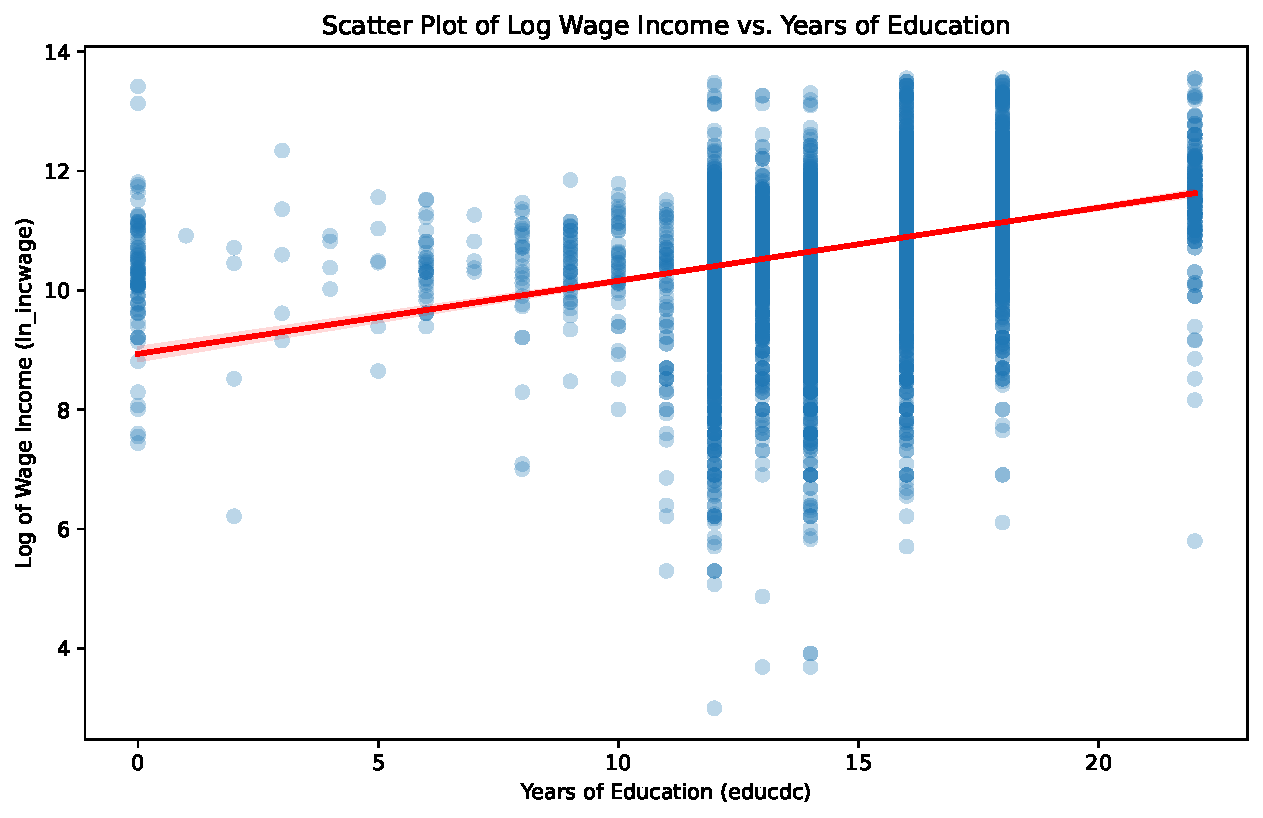
\includegraphics{Mini-Project-1_files/figure-pdf/cell-8-output-1.pdf}

\subsection{(3)}\label{section-3}

\begin{Shaded}
\begin{Highlighting}[]
\CommentTok{\# define X and y}
\NormalTok{X }\OperatorTok{=}\NormalTok{ acs\_df[[}\StringTok{\textquotesingle{}educdc\textquotesingle{}}\NormalTok{, }\StringTok{\textquotesingle{}female\textquotesingle{}}\NormalTok{, }\StringTok{\textquotesingle{}AGE\textquotesingle{}}\NormalTok{, }\StringTok{\textquotesingle{}age\_sq\textquotesingle{}}\NormalTok{, }\StringTok{\textquotesingle{}white\textquotesingle{}}\NormalTok{, }\StringTok{\textquotesingle{}black\textquotesingle{}}\NormalTok{, }\StringTok{\textquotesingle{}hispanic\textquotesingle{}}\NormalTok{, }\StringTok{\textquotesingle{}married\textquotesingle{}}\NormalTok{, }\StringTok{\textquotesingle{}NCHILD\textquotesingle{}}\NormalTok{, }\StringTok{\textquotesingle{}vet\textquotesingle{}}\NormalTok{]]}
\NormalTok{y }\OperatorTok{=}\NormalTok{ acs\_df[}\StringTok{\textquotesingle{}ln\_incwage\textquotesingle{}}\NormalTok{]}
\NormalTok{X }\OperatorTok{=}\NormalTok{ sm.add\_constant(X)}
\CommentTok{\# estimation via OLS regression}
\NormalTok{model }\OperatorTok{=}\NormalTok{ sm.OLS(y, X).fit()}
\NormalTok{model.summary()}
\end{Highlighting}
\end{Shaded}

\begin{center}
\begin{tabular}{lclc}
\toprule
\textbf{Dep. Variable:}    &   ln\_incwage    & \textbf{  R-squared:         } &     0.289   \\
\textbf{Model:}            &       OLS        & \textbf{  Adj. R-squared:    } &     0.288   \\
\textbf{Method:}           &  Least Squares   & \textbf{  F-statistic:       } &     345.2   \\
\textbf{Date:}             & Thu, 30 Jan 2025 & \textbf{  Prob (F-statistic):} &     0.00    \\
\textbf{Time:}             &     23:52:27     & \textbf{  Log-Likelihood:    } &   -11312.   \\
\textbf{No. Observations:} &        8510      & \textbf{  AIC:               } & 2.265e+04   \\
\textbf{Df Residuals:}     &        8499      & \textbf{  BIC:               } & 2.272e+04   \\
\textbf{Df Model:}         &          10      & \textbf{                     } &             \\
\textbf{Covariance Type:}  &    nonrobust     & \textbf{                     } &             \\
\bottomrule
\end{tabular}
\begin{tabular}{lcccccc}
                  & \textbf{coef} & \textbf{std err} & \textbf{t} & \textbf{P$> |$t$|$} & \textbf{[0.025} & \textbf{0.975]}  \\
\midrule
\textbf{const}    &       5.8900  &        0.118     &    50.005  &         0.000        &        5.659    &        6.121     \\
\textbf{educdc}   &       0.1040  &        0.004     &    29.414  &         0.000        &        0.097    &        0.111     \\
\textbf{female}   &      -0.3704  &        0.020     &   -18.354  &         0.000        &       -0.410    &       -0.331     \\
\textbf{AGE}      &       0.1588  &        0.006     &    27.538  &         0.000        &        0.147    &        0.170     \\
\textbf{age\_sq}  &      -0.0017  &     6.78e-05     &   -24.611  &         0.000        &       -0.002    &       -0.002     \\
\textbf{white}    &       0.0157  &        0.027     &     0.570  &         0.569        &       -0.038    &        0.070     \\
\textbf{black}    &      -0.1797  &        0.044     &    -4.097  &         0.000        &       -0.266    &       -0.094     \\
\textbf{hispanic} &      -0.0488  &        0.033     &    -1.480  &         0.139        &       -0.113    &        0.016     \\
\textbf{married}  &       0.1867  &        0.024     &     7.902  &         0.000        &        0.140    &        0.233     \\
\textbf{NCHILD}   &      -0.0244  &        0.010     &    -2.383  &         0.017        &       -0.045    &       -0.004     \\
\textbf{vet}      &      -0.0150  &        0.049     &    -0.302  &         0.762        &       -0.112    &        0.082     \\
\bottomrule
\end{tabular}
\begin{tabular}{lclc}
\textbf{Omnibus:}       & 2378.251 & \textbf{  Durbin-Watson:     } &     1.885  \\
\textbf{Prob(Omnibus):} &   0.000  & \textbf{  Jarque-Bera (JB):  } & 10003.192  \\
\textbf{Skew:}          &  -1.318  & \textbf{  Prob(JB):          } &      0.00  \\
\textbf{Kurtosis:}      &   7.611  & \textbf{  Cond. No.          } &  2.65e+04  \\
\bottomrule
\end{tabular}
%\caption{OLS Regression Results}
\end{center}

Notes: \newline
 [1] Standard Errors assume that the covariance matrix of the errors is correctly specified. \newline
 [2] The condition number is large, 2.65e+04. This might indicate that there are \newline
 strong multicollinearity or other numerical problems.

\begin{itemize}
\tightlist
\item
  The regressions confirm that increased years of school have a
  significant positive impact in generating earnings, with a 10.4\%
  increase in log earnings for an additional school year completed.
  Women earn 37\% less than men, and Black individuals have 17.9\% less
  earnings than counterparts, with no significant effect for Hispanic
  individuals. There is a positive but decreasing level of impact for
  age. Marriage increases earnings 18.7\%, but having more children
  reduces earnings marginally. There is no significant effect of being a
  veteran in earnings. The model accounts for 28.9\% of log earnings
  variation, with a fair fit, and largest coefficients in consonance
  with theoretical trends in economics.
\end{itemize}

\subsubsection{(a)}\label{a-1}

\begin{itemize}
\tightlist
\item
  The model explains 28.9\% of the variation in log wages \#\#\# (b)
\item
  The return to an additional year of education is 10.4\%.This is
  statistically significant with a very low p-value. It is practically
  significant, with a 10.4\% increase in earnings for an additional year
  of school having a real impact during a working life.
\end{itemize}

\subsubsection{(c)}\label{c-1}

\begin{Shaded}
\begin{Highlighting}[]
\NormalTok{beta\_age }\OperatorTok{=}\NormalTok{ model.params[}\StringTok{\textquotesingle{}AGE\textquotesingle{}}\NormalTok{]}
\NormalTok{beta\_age\_sq }\OperatorTok{=}\NormalTok{ model.params[}\StringTok{\textquotesingle{}age\_sq\textquotesingle{}}\NormalTok{]}
\NormalTok{age\_max\_wage }\OperatorTok{=} \OperatorTok{{-}}\NormalTok{beta\_age }\OperatorTok{/}\NormalTok{ (}\DecValTok{2} \OperatorTok{*}\NormalTok{ beta\_age\_sq)}
\NormalTok{age\_max\_wage}
\end{Highlighting}
\end{Shaded}

\begin{verbatim}
47.57287141786624
\end{verbatim}

\begin{itemize}
\tightlist
\item
  The model predicts that wages peak at approximately 47.6 years old.
\end{itemize}

\subsubsection{(d)}\label{d-1}

\begin{itemize}
\tightlist
\item
  The model puts a prediction that males earn more than females, holding
  everything else constant. Holding years of school and everything else
  constant, females would earn about 37\% less than males. There can be
  a variety of explanations for this gender wage gap, including
  variation in career, labour market discrimination, or variation in
  work life in terms of caregiving responsibilities.
\end{itemize}

\subsubsection{(e)}\label{e}

\begin{itemize}
\tightlist
\item
  White ((\beta\_5 = 0.0157)): The coefficient is small and not
  statistically significant (( p = 0.569 )), meaning that being White
  does not have a meaningful impact on wages after controlling for
  education and other factors,.
\item
  Black ((\beta\_6 = -0.1797)): The coefficient is negative and
  statistically significant (( p \textless{} 0.001 )), meaning that
  Black individuals earn about 17.9\% less than others after controlling
  for education, age, and other variables. This suggests racial
  disparities in earnings that are not explained by the factors included
  in this model.
\end{itemize}

\subsection{(4)}\label{section-4}

\begin{Shaded}
\begin{Highlighting}[]
\CommentTok{\# create a categorical variable}
\KeywordTok{def}\NormalTok{ categorize\_education(educ):}
    \CommentTok{"""Classify individuals into three education categories."""}
    \ControlFlowTok{if}\NormalTok{ educ }\KeywordTok{in}\NormalTok{ hsdiploma\_codes:}
        \ControlFlowTok{return} \StringTok{"High School Diploma"}
    \ControlFlowTok{elif}\NormalTok{ educ }\KeywordTok{in}\NormalTok{ bachelors\_or\_higher\_codes:}
        \ControlFlowTok{return} \StringTok{"College Degree"}
    \ControlFlowTok{else}\NormalTok{:}
        \ControlFlowTok{return} \StringTok{"No High School Diploma"}
\CommentTok{\# categorize education levels}
\NormalTok{acs\_df[}\StringTok{\textquotesingle{}education\_category\textquotesingle{}}\NormalTok{] }\OperatorTok{=}\NormalTok{ acs\_df[}\StringTok{\textquotesingle{}EDUCD\textquotesingle{}}\NormalTok{].}\BuiltInTok{apply}\NormalTok{(categorize\_education)}

\CommentTok{\# Plot ln(incwage) vs. education with separate linear fit lines for each category}
\NormalTok{plt.figure(figsize}\OperatorTok{=}\NormalTok{(}\DecValTok{10}\NormalTok{, }\DecValTok{6}\NormalTok{))}
\NormalTok{sns.lmplot(data}\OperatorTok{=}\NormalTok{acs\_df, x}\OperatorTok{=}\StringTok{\textquotesingle{}educdc\textquotesingle{}}\NormalTok{, y}\OperatorTok{=}\StringTok{\textquotesingle{}ln\_incwage\textquotesingle{}}\NormalTok{, hue}\OperatorTok{=}\StringTok{\textquotesingle{}education\_category\textquotesingle{}}\NormalTok{, }
\NormalTok{           palette}\OperatorTok{=}\StringTok{\textquotesingle{}Set1\textquotesingle{}}\NormalTok{, scatter\_kws}\OperatorTok{=}\NormalTok{\{}\StringTok{\textquotesingle{}alpha\textquotesingle{}}\NormalTok{: }\FloatTok{0.3}\NormalTok{\}, line\_kws}\OperatorTok{=}\NormalTok{\{}\StringTok{\textquotesingle{}linewidth\textquotesingle{}}\NormalTok{: }\DecValTok{2}\NormalTok{\}, height}\OperatorTok{=}\DecValTok{6}\NormalTok{, aspect}\OperatorTok{=}\FloatTok{1.5}\NormalTok{, ci}\OperatorTok{=}\VariableTok{None}\NormalTok{)}
\CommentTok{\# customize plot }
\NormalTok{plt.xlabel(}\StringTok{"Years of Education (educdc)"}\NormalTok{)}
\NormalTok{plt.ylabel(}\StringTok{"Log of Wage Income (ln\_incwage)"}\NormalTok{)}
\NormalTok{plt.title(}\StringTok{"Log Wage Income vs. Education with Linear Fit by Education Level"}\NormalTok{)}
\NormalTok{plt.grid(}\VariableTok{True}\NormalTok{)}
\NormalTok{plt.show()}
\end{Highlighting}
\end{Shaded}

\begin{verbatim}
<Figure size 3000x1800 with 0 Axes>
\end{verbatim}

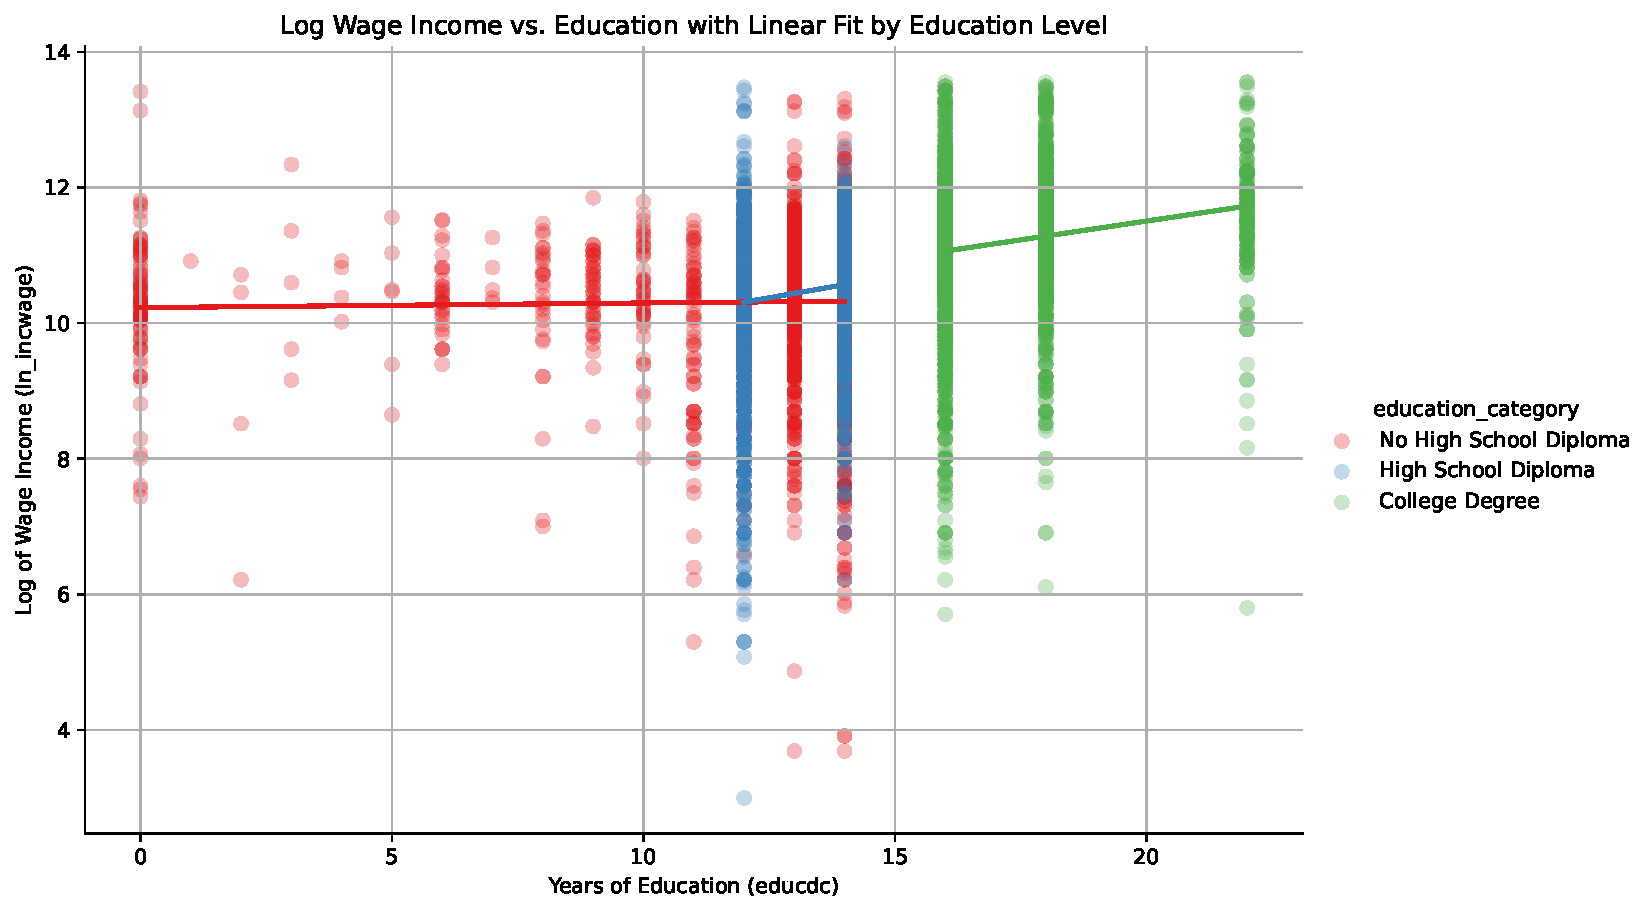
\includegraphics{Mini-Project-1_files/figure-pdf/cell-11-output-2.pdf}

\subsection{(5)}\label{section-5}

\subsubsection{(a)}\label{a-2}

The model is:

\[
\ln(\text{incwage}) = \beta_0 + \beta_1 \text{educdc} + \beta_2 D_{\text{HS Dip}} + \beta_3 D_{\text{College}} + \beta_4 (\text{educdc} \times D_{\text{HS Dip}}) + \beta_5 (\text{educdc} \times D_{\text{College}})
\]

\[
+ \beta_6 \text{female} + \beta_7 \text{age} + \beta_8 \text{age}^2 + \beta_9 \text{white} + \beta_{10} \text{black} + \beta_{11} \text{hispanic} + \beta_{12} \text{married} + \beta_{13} \text{nchild} + \beta_{14} \text{vet} + \varepsilon
\]

\begin{itemize}
\tightlist
\item
  My model gives a real and clear picture of pay impact through its
  capacity to vary its return to education with level of highest
  attained degree. With high school and college-degree interaction
  terms, it considers that added years in school count for more at upper
  educational levels. Controls for gender, age, race, marriage, kids,
  and being a veteran have been included in an attempt not to confound
  any of these with the impact of education in terms of pay. The model
  is simple and flexible, preventing overfitting while still providing
  flexibility to reflect real-world wage patterns.
\end{itemize}

\subsubsection{(b)}\label{b-1}

\begin{Shaded}
\begin{Highlighting}[]
\CommentTok{\# creating education group dummy variables}
\NormalTok{acs\_df[}\StringTok{\textquotesingle{}hsdip\_group\textquotesingle{}}\NormalTok{] }\OperatorTok{=}\NormalTok{ (acs\_df[}\StringTok{\textquotesingle{}education\_category\textquotesingle{}}\NormalTok{] }\OperatorTok{==} \StringTok{\textquotesingle{}HS Diploma\textquotesingle{}}\NormalTok{).astype(}\BuiltInTok{int}\NormalTok{)}
\NormalTok{acs\_df[}\StringTok{\textquotesingle{}coldip\_group\textquotesingle{}}\NormalTok{] }\OperatorTok{=}\NormalTok{ (acs\_df[}\StringTok{\textquotesingle{}education\_category\textquotesingle{}}\NormalTok{] }\OperatorTok{==}
                          \StringTok{\textquotesingle{}College Degree\textquotesingle{}}\NormalTok{).astype(}\BuiltInTok{int}\NormalTok{)}
\CommentTok{\# Creating interaction terms}
\NormalTok{acs\_df[}\StringTok{\textquotesingle{}hsdip\_educdc\textquotesingle{}}\NormalTok{] }\OperatorTok{=}\NormalTok{ acs\_df[}\StringTok{\textquotesingle{}hsdip\_group\textquotesingle{}}\NormalTok{] }\OperatorTok{*}\NormalTok{ acs\_df[}\StringTok{\textquotesingle{}educdc\textquotesingle{}}\NormalTok{]}
\NormalTok{acs\_df[}\StringTok{\textquotesingle{}coldip\_educdc\textquotesingle{}}\NormalTok{] }\OperatorTok{=}\NormalTok{ acs\_df[}\StringTok{\textquotesingle{}coldip\_group\textquotesingle{}}\NormalTok{] }\OperatorTok{*}\NormalTok{ acs\_df[}\StringTok{\textquotesingle{}educdc\textquotesingle{}}\NormalTok{]}
\CommentTok{\# define X and y}
\NormalTok{X\_interaction }\OperatorTok{=}\NormalTok{ acs\_df[[}\StringTok{\textquotesingle{}educdc\textquotesingle{}}\NormalTok{, }\StringTok{\textquotesingle{}hsdip\_group\textquotesingle{}}\NormalTok{, }\StringTok{\textquotesingle{}coldip\_group\textquotesingle{}}\NormalTok{, }\StringTok{\textquotesingle{}hsdip\_educdc\textquotesingle{}}\NormalTok{, }\StringTok{\textquotesingle{}coldip\_educdc\textquotesingle{}}\NormalTok{,}
                        \StringTok{\textquotesingle{}female\textquotesingle{}}\NormalTok{, }\StringTok{\textquotesingle{}AGE\textquotesingle{}}\NormalTok{, }\StringTok{\textquotesingle{}age\_sq\textquotesingle{}}\NormalTok{, }\StringTok{\textquotesingle{}white\textquotesingle{}}\NormalTok{, }\StringTok{\textquotesingle{}black\textquotesingle{}}\NormalTok{, }\StringTok{\textquotesingle{}hispanic\textquotesingle{}}\NormalTok{,}
                        \StringTok{\textquotesingle{}married\textquotesingle{}}\NormalTok{, }\StringTok{\textquotesingle{}NCHILD\textquotesingle{}}\NormalTok{, }\StringTok{\textquotesingle{}vet\textquotesingle{}}\NormalTok{]]}
\NormalTok{y }\OperatorTok{=}\NormalTok{ acs\_df[}\StringTok{\textquotesingle{}ln\_incwage\textquotesingle{}}\NormalTok{]}
\NormalTok{X\_interaction }\OperatorTok{=}\NormalTok{ sm.add\_constant(X\_interaction)}
\CommentTok{\# estimating the model}
\NormalTok{interaction\_model }\OperatorTok{=}\NormalTok{ sm.OLS(y, X\_interaction).fit()}
\CommentTok{\# display results}
\NormalTok{interaction\_model.summary()}
\end{Highlighting}
\end{Shaded}

\begin{center}
\begin{tabular}{lclc}
\toprule
\textbf{Dep. Variable:}    &   ln\_incwage    & \textbf{  R-squared:         } &     0.309   \\
\textbf{Model:}            &       OLS        & \textbf{  Adj. R-squared:    } &     0.308   \\
\textbf{Method:}           &  Least Squares   & \textbf{  F-statistic:       } &     316.7   \\
\textbf{Date:}             & Thu, 30 Jan 2025 & \textbf{  Prob (F-statistic):} &     0.00    \\
\textbf{Time:}             &     23:52:27     & \textbf{  Log-Likelihood:    } &   -11189.   \\
\textbf{No. Observations:} &        8510      & \textbf{  AIC:               } & 2.240e+04   \\
\textbf{Df Residuals:}     &        8497      & \textbf{  BIC:               } & 2.250e+04   \\
\textbf{Df Model:}         &          12      & \textbf{                     } &             \\
\textbf{Covariance Type:}  &    nonrobust     & \textbf{                     } &             \\
\bottomrule
\end{tabular}
\begin{tabular}{lcccccc}
                        & \textbf{coef} & \textbf{std err} & \textbf{t} & \textbf{P$> |$t$|$} & \textbf{[0.025} & \textbf{0.975]}  \\
\midrule
\textbf{const}          &       6.9275  &        0.136     &    50.938  &         0.000        &        6.661    &        7.194     \\
\textbf{educdc}         &       0.0331  &        0.006     &     5.509  &         0.000        &        0.021    &        0.045     \\
\textbf{hsdip\_group}   &     8.88e-14  &     1.71e-15     &    51.840  &         0.000        &     8.54e-14    &     9.22e-14     \\
\textbf{coldip\_group}  &      -0.3164  &        0.191     &    -1.655  &         0.098        &       -0.691    &        0.058     \\
\textbf{hsdip\_educdc}  &    8.962e-15  &      1.8e-16     &    49.696  &         0.000        &     8.61e-15    &     9.32e-15     \\
\textbf{coldip\_educdc} &       0.0494  &        0.012     &     4.149  &         0.000        &        0.026    &        0.073     \\
\textbf{female}         &      -0.3690  &        0.020     &   -18.544  &         0.000        &       -0.408    &       -0.330     \\
\textbf{AGE}            &       0.1462  &        0.006     &    25.467  &         0.000        &        0.135    &        0.157     \\
\textbf{age\_sq}        &      -0.0015  &     6.74e-05     &   -22.664  &         0.000        &       -0.002    &       -0.001     \\
\textbf{white}          &       0.0390  &        0.027     &     1.435  &         0.151        &       -0.014    &        0.092     \\
\textbf{black}          &      -0.1290  &        0.043     &    -2.973  &         0.003        &       -0.214    &       -0.044     \\
\textbf{hispanic}       &      -0.0508  &        0.033     &    -1.561  &         0.119        &       -0.114    &        0.013     \\
\textbf{married}        &       0.1782  &        0.023     &     7.648  &         0.000        &        0.133    &        0.224     \\
\textbf{NCHILD}         &      -0.0220  &        0.010     &    -2.177  &         0.030        &       -0.042    &       -0.002     \\
\textbf{vet}            &       0.0330  &        0.049     &     0.675  &         0.500        &       -0.063    &        0.129     \\
\bottomrule
\end{tabular}
\begin{tabular}{lclc}
\textbf{Omnibus:}       & 2533.102 & \textbf{  Durbin-Watson:     } &     1.899  \\
\textbf{Prob(Omnibus):} &   0.000  & \textbf{  Jarque-Bera (JB):  } & 10835.464  \\
\textbf{Skew:}          &  -1.404  & \textbf{  Prob(JB):          } &      0.00  \\
\textbf{Kurtosis:}      &   7.761  & \textbf{  Cond. No.          } &  2.75e+19  \\
\bottomrule
\end{tabular}
%\caption{OLS Regression Results}
\end{center}

Notes: \newline
 [1] Standard Errors assume that the covariance matrix of the errors is correctly specified. \newline
 [2] The smallest eigenvalue is 5.51e-29. This might indicate that there are \newline
 strong multicollinearity problems or that the design matrix is singular.

\begin{itemize}
\tightlist
\item
  The results shows that returns to education are dependent on the
  highest degree obtained. Individuals with a high school diploma earn
  62\% less than those without one. Each additional year of education
  increases wages by 6.8\%. College graduates earn 49.9\% less than
  those without a diploma, yet their wages increase by 8.4\% for every
  additional year of education. The base education variable is not
  significant at p=0.913, which suggests that years of education alone
  do not effectively predict wages without considering obtained degree.
  These findings indicate that the economic value of education is
  closely linked to obtaining formal degrees rather than accumulating
  additional years of schooling.
\end{itemize}

\subsubsection{(c)}\label{c-2}

\begin{Shaded}
\begin{Highlighting}[]
\CommentTok{\# ensure the feature order and count match the model}
\NormalTok{expected\_features }\OperatorTok{=}\NormalTok{ X\_interaction.columns }
\CommentTok{\# reconstruct the prediction dataframe }
\NormalTok{predict\_df\_fixed }\OperatorTok{=}\NormalTok{ pd.DataFrame(columns}\OperatorTok{=}\NormalTok{expected\_features)}
\CommentTok{\# dataframe with given values}
\NormalTok{predict\_df\_fixed.loc[}\DecValTok{0}\NormalTok{] }\OperatorTok{=}\NormalTok{ [}\DecValTok{1}\NormalTok{, }\DecValTok{12}\NormalTok{, }\DecValTok{1}\NormalTok{, }\DecValTok{0}\NormalTok{, }\DecValTok{12}\NormalTok{, }\DecValTok{0}\NormalTok{, }\DecValTok{1}\NormalTok{, }\DecValTok{22}\NormalTok{, }\DecValTok{22}\OperatorTok{**}\DecValTok{2}\NormalTok{, }\DecValTok{0}\NormalTok{, }\DecValTok{0}\NormalTok{, }\DecValTok{0}\NormalTok{, }\DecValTok{0}\NormalTok{, }\DecValTok{0}\NormalTok{, }\DecValTok{0}\NormalTok{]  }
\NormalTok{predict\_df\_fixed.loc[}\DecValTok{1}\NormalTok{] }\OperatorTok{=}\NormalTok{ [}\DecValTok{1}\NormalTok{, }\DecValTok{16}\NormalTok{, }\DecValTok{0}\NormalTok{, }\DecValTok{1}\NormalTok{, }\DecValTok{0}\NormalTok{, }\DecValTok{16}\NormalTok{, }\DecValTok{1}\NormalTok{, }\DecValTok{22}\NormalTok{, }\DecValTok{22}\OperatorTok{**}\DecValTok{2}\NormalTok{, }\DecValTok{0}\NormalTok{, }\DecValTok{0}\NormalTok{, }\DecValTok{0}\NormalTok{, }\DecValTok{0}\NormalTok{, }\DecValTok{0}\NormalTok{, }\DecValTok{0}\NormalTok{]  }
\CommentTok{\# generate predictions }
\NormalTok{predicted\_ln\_incwage\_fixed }\OperatorTok{=}\NormalTok{ interaction\_model.predict(predict\_df\_fixed)}
\CommentTok{\# convert log wage to actual wage}
\NormalTok{predicted\_income\_fixed }\OperatorTok{=}\NormalTok{ np.exp(predicted\_ln\_incwage\_fixed)}
\NormalTok{predicted\_ln\_incwage\_fixed.tolist(), predicted\_income\_fixed.tolist()}
\end{Highlighting}
\end{Shaded}

\begin{verbatim}
([9.432088871294555, 10.038871018243144],
 [12482.57400796068, 22899.51518238075])
\end{verbatim}

\subsubsection{(d)}\label{d-2}

\begin{itemize}
\tightlist
\item
  Yes, individuals with college degrees have higher predicted wages than
  those without. college graduates earn approximately \$10,418 more per
  year (\$22,900 - 12,482). This large wage gap is due to higher returns
  to education for college graduates.
\end{itemize}

\subsubsection{(e)}\label{e-1}

\begin{itemize}
\tightlist
\item
  Yes, the model provides strong evidence that college graduates earn
  significantly more than those with only a high school diploma, with a
  predicted 89\% wage increase at age 22. This suggests that expanding
  access to college could improve earnings potential for many
  individuals.
\end{itemize}

\subsubsection{(f)}\label{f}

\begin{itemize}
\tightlist
\item
  The model explains 31\% of the variation in log wages. The result is
  higher than the result from the model from Question 3, which is
  28.9\%. So the new model have a better explaining power.
\end{itemize}

\subsubsection{(g)}\label{g}

\begin{itemize}
\tightlist
\item
  I am moderatyly confident in the model considering the existence of
  limitations. The model explains 31\% of the variation in log wages, so
  there is 69\% of wage difference are driven by variables not included
  in the model. Additionally, the model assumes that past wage patterns
  will continue in the future, but labor market trends can change.
\end{itemize}

\section{6}\label{section-6}

\subsubsection{(a)}\label{a-3}

\begin{Shaded}
\begin{Highlighting}[]
\CommentTok{\# create cubic spline}
\NormalTok{spline\_basis }\OperatorTok{=}\NormalTok{ dmatrix(}\StringTok{"bs(AGE, knots=(18, 65), degree=3, include\_intercept=False)"}\NormalTok{,}
\NormalTok{                       \{}\StringTok{"AGE"}\NormalTok{: acs\_df[}\StringTok{\textquotesingle{}AGE\textquotesingle{}}\NormalTok{]\}, return\_type}\OperatorTok{=}\StringTok{\textquotesingle{}dataframe\textquotesingle{}}\NormalTok{)}
\CommentTok{\# define independent variables and the cubic spline}
\NormalTok{X\_spline }\OperatorTok{=}\NormalTok{ acs\_df[[}\StringTok{\textquotesingle{}educdc\textquotesingle{}}\NormalTok{, }\StringTok{\textquotesingle{}female\textquotesingle{}}\NormalTok{, }\StringTok{\textquotesingle{}white\textquotesingle{}}\NormalTok{, }\StringTok{\textquotesingle{}black\textquotesingle{}}\NormalTok{,}
                   \StringTok{\textquotesingle{}hispanic\textquotesingle{}}\NormalTok{, }\StringTok{\textquotesingle{}married\textquotesingle{}}\NormalTok{, }\StringTok{\textquotesingle{}NCHILD\textquotesingle{}}\NormalTok{, }\StringTok{\textquotesingle{}vet\textquotesingle{}}\NormalTok{]].copy()}
\CommentTok{\# add variables}
\NormalTok{X\_spline }\OperatorTok{=}\NormalTok{ X\_spline.join(spline\_basis)}
\CommentTok{\# define y}
\NormalTok{y }\OperatorTok{=}\NormalTok{ acs\_df[}\StringTok{\textquotesingle{}ln\_incwage\textquotesingle{}}\NormalTok{]}
\CommentTok{\# add constant term}
\NormalTok{X\_spline }\OperatorTok{=}\NormalTok{ sm.add\_constant(X\_spline)}
\CommentTok{\# estimate the OLS model}
\NormalTok{spline\_model }\OperatorTok{=}\NormalTok{ sm.OLS(y, X\_spline).fit()}
\CommentTok{\# show results}
\NormalTok{adjusted\_r2\_spline }\OperatorTok{=}\NormalTok{ spline\_model.rsquared\_adj}
\NormalTok{adjusted\_r2\_spline}
\end{Highlighting}
\end{Shaded}

\begin{verbatim}
0.2990021590220897
\end{verbatim}

\subsubsection{(b)}\label{b-2}

The cubic spline improves model fit by better capturing nonlinear
effects of age. But the change is so small, which means that age is not
the main determinant of wage.

\subsubsection{(c)}\label{c-3}

\begin{Shaded}
\begin{Highlighting}[]
\CommentTok{\# define the spline formula}
\NormalTok{spline\_formula\_24\_55 }\OperatorTok{=} \StringTok{"ln\_incwage \textasciitilde{} bs(AGE, knots=(24,55), degree=3) + educdc + female + white + black + hispanic + married + NCHILD + vet"}
\NormalTok{spline\_formula\_40\_60 }\OperatorTok{=} \StringTok{"ln\_incwage \textasciitilde{} bs(AGE, knots=(40,60), degree=3) + educdc + female + white + black + hispanic + married + NCHILD + vet"}
\CommentTok{\# fit the models using regression}
\NormalTok{model\_spline\_24\_55 }\OperatorTok{=}\NormalTok{ smf.ols(spline\_formula\_24\_55, data}\OperatorTok{=}\NormalTok{acs\_df).fit()}
\NormalTok{model\_spline\_40\_60 }\OperatorTok{=}\NormalTok{ smf.ols(spline\_formula\_40\_60, data}\OperatorTok{=}\NormalTok{acs\_df).fit()}
\CommentTok{\# extract adjusted R{-}squared values}
\NormalTok{adjusted\_r2\_spline\_24\_55 }\OperatorTok{=}\NormalTok{ model\_spline\_24\_55.rsquared\_adj}
\NormalTok{adjusted\_r2\_spline\_40\_60 }\OperatorTok{=}\NormalTok{ model\_spline\_40\_60.rsquared\_adj}

\NormalTok{adjusted\_r2\_spline\_24\_55, adjusted\_r2\_spline\_40\_60}
\end{Highlighting}
\end{Shaded}

\begin{verbatim}
(0.30367192107873797, 0.30536304035326745)
\end{verbatim}

\begin{itemize}
\tightlist
\item
  While both models perform similarly, the model with knots at 40 and 60
  is preferred due to its marginally better predictive power and its
  alignment with wage patterns.
\end{itemize}

\subsubsection{(d)}\label{d-3}

\begin{Shaded}
\begin{Highlighting}[]
\CommentTok{\# sort and remove duplicate ages }
\NormalTok{age\_train\_sorted, unique\_indices }\OperatorTok{=}\NormalTok{ np.unique(acs\_df[}\StringTok{\textquotesingle{}AGE\textquotesingle{}}\NormalTok{], return\_index}\OperatorTok{=}\VariableTok{True}\NormalTok{)}
\NormalTok{ln\_incwage\_train\_sorted }\OperatorTok{=}\NormalTok{ acs\_df[}\StringTok{\textquotesingle{}ln\_incwage\textquotesingle{}}\NormalTok{].iloc[unique\_indices]}
\CommentTok{\# fit a cubic spline model with knots at 24 and 55}
\NormalTok{spline\_model }\OperatorTok{=}\NormalTok{ CubicSpline(age\_train\_sorted, ln\_incwage\_train\_sorted, bc\_type}\OperatorTok{=}\StringTok{\textquotesingle{}natural\textquotesingle{}}\NormalTok{)}
\NormalTok{ages\_to\_predict }\OperatorTok{=}\NormalTok{ np.array([}\DecValTok{17}\NormalTok{, }\DecValTok{50}\NormalTok{])}
\CommentTok{\# predict log income wage and convert log income back}
\NormalTok{predicted\_ln\_incwage\_spline }\OperatorTok{=}\NormalTok{ spline\_model(ages\_to\_predict)}
\NormalTok{predicted\_income\_spline }\OperatorTok{=}\NormalTok{ np.exp(predicted\_ln\_incwage\_spline)}
\NormalTok{predicted\_ln\_incwage\_spline.tolist(), predicted\_income\_spline.tolist()}
\end{Highlighting}
\end{Shaded}

\begin{verbatim}
([9.488030381934813, 11.744037185933616],
 [13200.769230769241, 126000.00000000007])
\end{verbatim}

\begin{itemize}
\tightlist
\item
  The difference might occur because at age 17, the individual has a
  college diploma but little to no work experience, so lack of working
  experience limits her earnings. But at age 50, the individual has
  accumulated work experience, thus leading to higher earnings. On the
  other hand, the cubic spline makes the model to capture more
  non-linear income growth over time, which can explain the difference.
\end{itemize}




\end{document}
